%% This is a document discussing a decision to completely decouple the 
%% graphical subsystem of the designer from the subsystem of the VT (verification tools).
%%
%% This document is the main document: compile with xelatex to get the complete pdf.
%%

\documentclass[a4paper,11pt,final]{article}

\usepackage[english]{babel}
\usepackage{graphicx}
\usepackage{hyperref}
\hypersetup{ colorlinks = true, citecolor = blue,linkcolor = blue }
\usepackage[a4paper]{geometry}
\usepackage{titlesec}% added to change section headers, see newcommand definition.
\usepackage{xspace}

\bibliographystyle{alpha}

\author{ABI team 33\\(Stefan Versluys, Guus Bonnema, Jeroen Kleijn)}

\date{20/02/2015}

\title{\color{blue}VT - XMD integration}

\newcommand{\w}[1]{\texttt{#1}\xspace}
\newcommand{\xmas}{\textsc{xmas}\xspace}%
\newcommand{\xmd}{\textsc{xmd}\xspace}%
\newcommand{\vt}{\textsc{vt}\xspace}%
\newcommand{\qt}{\textsc{Qt}\xspace}%
\newcommand{\qtquick}{\textsc{QtQuick}\xspace}%
\newcommand{\qml}{\textsc{Qt}\xspace}%
\newcommand{\cpp}{\textsc{C++}\xspace}%


\begin{document}
\selectlanguage{english}

\maketitle

\begin{abstract}

	* Why did we write this document? 
	* What does it cover?
	* How to read it? 
	
	This document explains why and in what manner the team decided 
	to decouple the designer subsystem \xmd and the \vt subsystem.
	The contents documents the background, the problem, the decison
	and the motivation for the decision, and finally the detailed 
	considerations that lead to the decision.
	
	The final structure of the subsystems (the diagram) will be part of 
	the system documentation.
\end{abstract}

%% Modification history

\begin{tabular}{|l|l|p{20em}|}
\hline 
\multicolumn{3}{|c|}{\bf Modification History}\\\hline
Stefan Versluys & 17-02-2015 & Initial discussion formulation \\\hline 
Guus Bonnema & 20-02-2015 & Transformation to decision document \\\hline 
\end{tabular} 

\maketitle

\tableofcontents

\section{Problem background and description}

\paragraph{Background}
During the planning phase of the project, the customer requested that
the designer be integrated with the verification tools in a way that
should be transparant to the user. Seamless integration should be the
appearance, whether or not the technical integration would be seamless.

For that reason the team experimented with different forms of integration
and finally reached the stage where we could formulate the alternatives
that we deem viable and decide.

This document describes in summary which alternatives we compared, what
we decided and what our motivation was. 

\paragraph{Description and alternatives}
Once we decided to switch to \qt as the user interface toolkit, we were
confronted with 3 different technologies that \qt uses to
implement a user interface: GraphicsView, \qtquick1 and \qtquick2. The 
decision at the time was to use \qtquick2 and the related replacement
for javascript \qml (referred to as \qml2). 

Immediately after this decision we started studying the interface between 
\qml and \cpp in order to interface the \xmd subsystem (the designer) with
the \vt subsystem (verification tools). The experimentation that followed
lead us to three alternative implementations that we partially implemented
before reaching the conclusion formulated below.

We considered the following alternatives:

\begin{description}
	\item[\cpp parser] In this alternative we communicate from
	the designer to a mapper class that catches each signal for creation
	of a component on the designer and translates it into the currently
	existing structure (\w{xmas.h}). This implies complete and integral
	coupling of the \xmd subsystem and the \vt subsystem through this
	mapper class. Also, the flat json designed in previous activities were
	to be amended for the new designer capabilities including graphical
	data requirements.
	
	\item[Partial \cpp parser and javascript parser] This alternative
	implies two structures that contain the network design: one for
	the designer and one for the \vt subsystem which is the existing 
	\w{fjson} structure. This implies translation of one datastructure 
	to another from the mapper class but limits the exposure of graphical 
	needs of the designer to the verification structure.
	
	\item[Full javascript parser] This alternatives implies two structures
	as well, but uses the \w{fjson} text stream as interface between the
	two subsystems. This implies that there is no other coupling between
	the \xmd subsystem and the \vt subsystem and no modifications to the
	\vt system are necessary other than those needed to run and compile on
	all specified platforms. 
\end{description}

\begin{figure}[here]
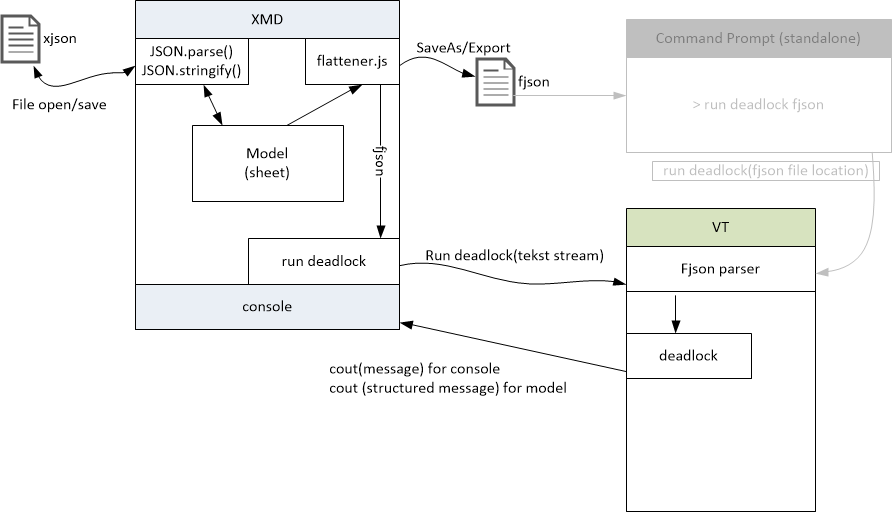
\includegraphics[width=1.0\textwidth]{xmd2vt}
\caption{Diagram for \textit{Full javascript parser}}
\label{fig:fulljavascriptparser}
\end{figure}


\section{Decision and motivation}

Due to the massive advantages that the loose coupling of the alternative 
\textit{Full javascript parser} offers, we decided in favour of this alternative. 

\section{Implications for future changes}

The decision implies that \vt development is relatively independant of 
designer development. Any changes to the interface of the \w{fjson} structure
impacts both subsystems, but all other changes are independent.

Additionally we still need a mechanism to start and stop verification tools, track
the error responses and we need to couple the verification tools executables into
the designer without creating a development dependency. 


\section{Details of the original discussion for VT - XMD integration}

\paragraph{Subject for discussion}
This discussion concerns the way verification tools (VT) can be integrated
into or interact with the Xmas Model Designer (XMD). There are several
options but not clear which is the best, because of conflicts in their
requirements \& specifications, additional risks, increase of complexity
and fade of basic rules concerning separation. 


\paragraph{vt requirements \& specification which affect integration decision:}
\begin{itemize}
\item The vt'’s are written in pure c++ because they can run on platforms without any specific software tools.
\item vt'’s their mayor key is performance.
\item The vt parser can handle a flat json structured file.
\item The vt parser cannot handle composites.
\item The vt parser feeds the vt model and has no GUI properties.
\item The vt'’s can be started and get their input via the command prompt. (standalone)
\item The vt'’s can be started and get their input via the designer tool.
\item The vt'’s structure is complex because it has to execute an algorithm and has to know
	about the message details plus its focus is performance and not maintainability.
\item The vt'’s give feedback via the standard output
\end{itemize}

\paragraph{xmd requirements \& specification which affect integration decision:}
\begin{itemize}
\item xmd is written in qml/c++ with Qt classes which gains development speed, fancy GUI, easy scripting.
\item xmd must handle composites.
\item xmd its major key is maintainability
\item Composites can be inside other composites and implies a hierarchical structure
\item xmd needs a hierarchical json parser
\item xmd needs GUI specific component properties like x,y,orientation
\item xmd doesn'’t need vt specific component model data structures.
\item xmd must be pure GUI and doesn'’t need to know about complex vt structures
\item Ideally vt integration in xmd must be purely interaction,  as if they are one thing for the xmd user but technically totally separated.
\item xmd must show the vt'’s feedback in the console (normal text message)
\item xmd can show the vt'’s result in the model (structured text message)
\end{itemize}

\paragraph{Team:}
\begin{itemize}
\item vt'’s are out of scope.
\item Modifying vt'’s parser and the structure to pass additional data is a risk:
	\begin{itemize}
	\item planning : complexity gains time?
	\item focus is xmd : loss of vt requirements/correctness?
	\item Because of OU changes, Bernard cannot be part of the team as developper.
	\item xmd interaction is done through the whole structure and makes vt and xmd very dependent from each other.
	\item Because of this dependence a change at the vt side can harm xmd and vice versa and breaks the maintainability rule.
		The same holds if changing xmd which can decrease vt its performance. 
	\end{itemize}
\item	Using the vt parser and underlaying data structure extends its complexity
	into xmd which conflicts with xmd's maintainability requirement.
\item Bernard: use only one data model, easier to maintain.
\item Bernard: vt has a parser you can use it.
\item Freeks concern of diving too deep into the vt'’s because of too many risks and getting out of scope. (see email)
\end{itemize}

\section{Options}
\paragraph{}

\paragraph{vt pure c++ parser only:}
\begin{itemize}
\item +/+ only one file type for \xmd and \vt
\item +/- one parser and model : not an advantage see remarks (*)
\item -/- flattening must be done at \vt side in pure c++
\item -/- XMD depends on the \vt parser and complex \vt structure for mapping.
\item -/- increased exposure to change issues between \vt and \xmd.
\item -/- \vt structure mixed with GUI parameters (x,y,orientation,scale,..)
\item -/- \vt parser and structure modification = risk + out of scope
\item -/- current fjson files not compatible anymore = loss of test references
\item -/- composites need to be handled/flattened in \vt parser
\item -/- handling composite file locations, \xmd vs. \vt standalone on a pure platform
\item -/- id references of components or ports can become inconsistent.
\end{itemize}

(*)The advantage of having a parser already is not an issue because in
javascript a parser is one line of code.
The disadvantage of having to modify two parsers /models isn'’t an issue
because in javascript, modifying is just adding a JSON field.
If vt and xmd are independent, a modification of the xmd parser doesn'’t lead to
a vt parser modification if it'’s just about a GUI parameter. A flattener only pick
items which are relevant for the vt'’s.

\paragraph{xmd Javascript parser + vt dependent:}
\begin{itemize}
\item +/+ \xmd can have its own json structure with GUI specific parameters
\item +/+ flattening can be done outside VT, no need to use pure c++
\item +/+ fjson stays compatible
\item +/+ no need to modify \vt to handle composites (parsing+flattening)
\item +/+ composite handling not necessary in \vt for this project.
\item -/- two file types , one hierarchical json and one fjson. Same as the current WickedXmas.
\item -/- mapping for flattening is still done via \vt parser/data, meaning complex \vt data structures into flattener.
\item -/- a designer must hand over flat files to a verifier using \vt as stand alone. 
\end{itemize}

\paragraph{xmd Javascript parser + vt independent:}
\begin{itemize}
\item same advantages as previous
<<<<<<< HEAD
\item +/+ flattening done totally independant in e.g. Javascript , no need to know \vt 
		data structures.  No mapping.
\item +/+ \xmd and \vt are completely independent, only the fjson structure is common.
\item +/- flat structure in \xmd must match \vt flat structure , but in javascript
	very small modification. Much easier than adopt mapping to complex datastructures.
\item +/+ flattening in the design tool can be used to see if there are no cycles before these are send to de VT’s
\item +/+ very low risk, only the fjson structure must match
\item +/+ no need of complex mapping code in designer, pure compact, robust and easy javascript
\item -/- two file types xmd + fjson
\item -/- \xmd needs and SaveAs or export function to fjson , so \vt’s can run models as standalone
\end{itemize}


Figure~\ref{fig:fulljavascriptparser} is a setup where \vt and \xmd are totally independent
but can interact with each other as if they are one thing. By this \xmd can keep
its maintainability and apart from minor changes \vt stays untouched.
The fjson structure is the only key they have in common.

\paragraph{Example of JSON in javascript:}\

\begin{figure}[here]
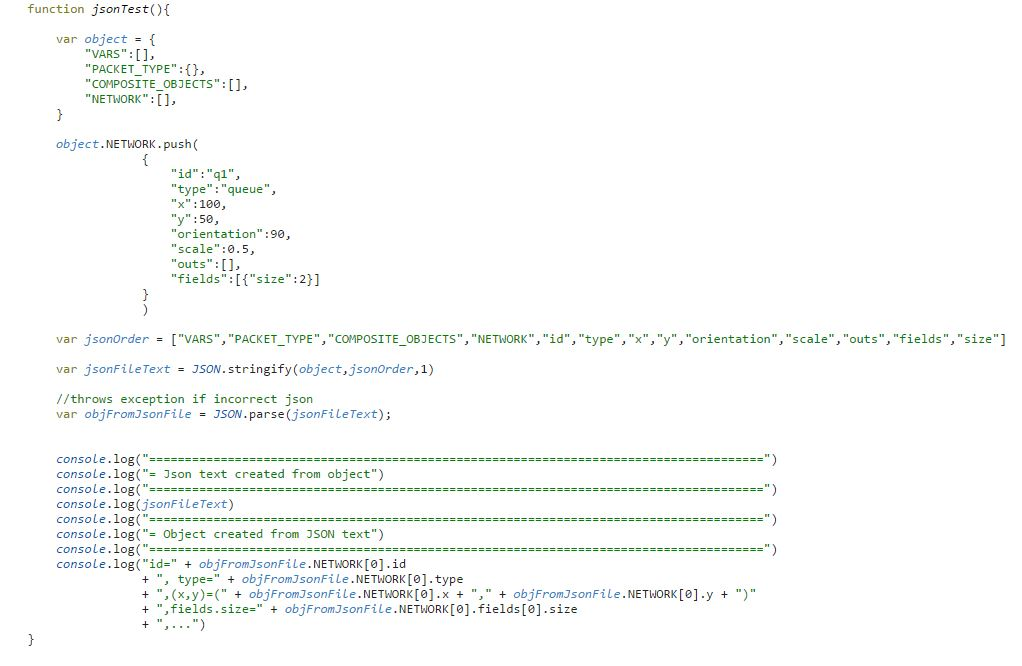
\includegraphics[width=0.90\textwidth]{js_json}
\caption{Javascript json example}
\label{fig:js_json}
\end{figure}
Figure~\ref{fig:js_json} is a javascript function creating a json structure
which is compatible with the current fjson.

\paragraph{}
\begin{figure}[here]
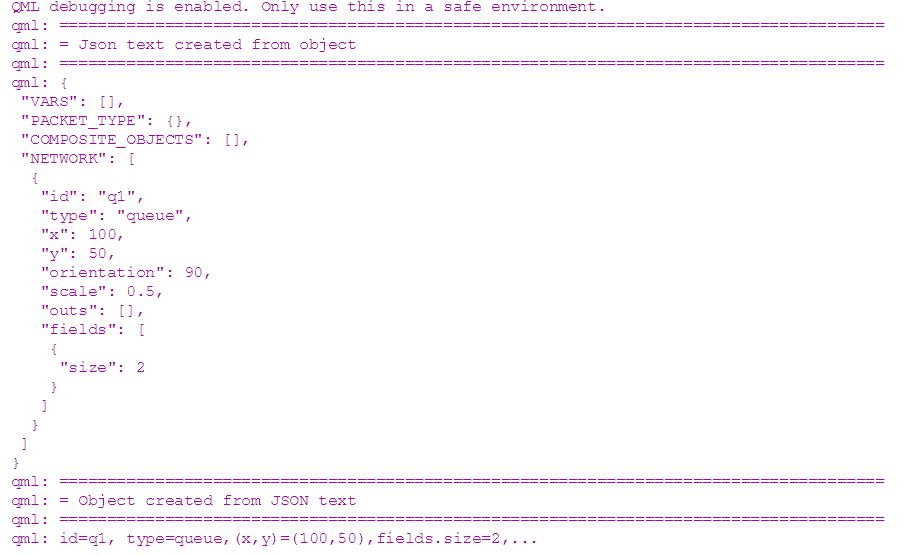
\includegraphics[width=0.90\textwidth]{js_json_result}
\caption{Javascript json console output}
\label{fig:js_json_result}
\end{figure}
Figure~\ref{fig:js_json_result} result of executing previous javascript function.

\section{Conclusion}
The third option, meaning xmd completely independent, is the most
appropriate choice. It has a low risk and maximum independancy,
the latter is important to prevent fading their major keys into
each other, certainly because these keys are conflicting.
During the last meeting with our customer, about reusing
the vt'’s parser and use one data model for the whole application,
was a good advice at first sight. Following that way we're
now at a point where we bump into several problems.
Vt and xmd are based on totally different requirements and by mixing
those two applications together we create a big risk. The risk
that we have to adopt vt too much that we will run out of time, we
have two iterations left.
Vt its source is complex, we noticed that even adding a simple parameter 
is not that easy and we still need to do a lot. Work like saving a file via
the vt structures and parser, composites and the flattener in pure c++.

\paragraph{}

In option three, vt only need some small adjustments and xmd will become
completely independent.
The risk that during maintenance the customer has to modify two
parsers doesn'’t exist. Parsing Json in Javascript is very easy compared
to modification in complex mappings between xmd and vt.
The same holds for the data model , there will be only one and that'’s the
original vt data model because xmd doesn'’t need to know about it.
Xmd only knows its graphical model as now in qml or Javascript.
Having two application doing an other thing with the same kind of data
without using the same libraries or whatever is a common thing.
E.g. zip is such a common structure or something like Qt Creator
which knows about the c++ syntax but only triggers an external
compiler is very similar to this application.

\paragraph{What has to be done at vt if option three is chosen?}
\begin{itemize}
\item A vt can be started with a fjson file argument.
		E.g. deadlock -f:2queues.fjson
\item A vt can be started with a fjson text argument
		E.g. deadlock -t:{fjson text stream out of xmd flattener}
\item A vt can be stopped
\item A vt can send messages to the standard output redirected to xmd its log.
\item A vt can send results to the xmd model as structured text
		E.g. cout([result] q1:5,q3:6.........)
\item A vt can send its status on request E.g. deadlock -status
\end{itemize}

\paragraph{What we don'’t have to do in vt if option three is chosen?}
\begin{itemize}
\item Writing a flattener in pure c++ which has to be integrated
	in the vt parser because of the composites.
\item Handling composites in vt. E.g. what about the composite 
	file locations? For a xmd user it can be different than for
	a vt user who's working standalone on a naked platform.
\item facing the risk of getting out of scope.
\item facing the risk of creating bugs in the vt software.
\item facing the risk of degrading vt'’s performance.
\item having the current fjson structure become incompatible,
	meaning loss of test reference.
\end{itemize}

\paragraph{What have to be changed in xmd?}
\begin{itemize}
\item Writing a flattener in Javascript.
\item Remove complex mapping with vt structures.
\item Create a JSON object of the canvas (sheet).
\item Write a process starter with text stream. (QProcess,stdin/out ? must be pure c++ compatible at the vt side)
\item redirect vt its output to the log
\end{itemize}


By this we can focus on finalise and fine tune the project during our last two iterations
and write documentation which e.g. describes how a customer can add a
new kind of primitive in xmd javascript or how a user can change fjson
structure with the JSON parser from javascript.

Of course the choice of our customer has the highest priority but
at least the customer must be aware of these consequences.

\end{document}
